\documentclass[11pt]{ieeeconf}
\usepackage{graphicx}
\usepackage{float}
\usepackage{lettrine}
\usepackage{caption}
\usepackage{url}


\newcommand\blfootnote[1]{%
  \begingroup
  \renewcommand\thefootnote{}\footnote{#1}%
  \addtocounter{footnote}{-1}%
  \endgroup
}

\title{Bumper Car Sumo}
\author{Jaden Simon - simonjaden223@gmail.com \\ \and
	   Melvin Bosnjak - meco0597@gmail.com \\ \and
	   Daniel Humeniuk - d.humeniuk@utah.edu \\ \and
	   http://bumpercarsumo.weebly.com/}

%Herein is our final report

%Professor Stevens' requirements for the report bellow

%Make sure you take time for your technical documentation! The final technical report can be completed the week following your project demonstration. Don't forget to plan for that! The final technical document will be written in LaTeX and will require formatting as the two column IEEE conference or journal paper as was done in 3991.

%This aspect of the project is critical to ensure that you are communicating well with the instructor as to the status of your project. This portion of the grade will be based on the weekly logs and team meetings that you have with the instructor. It is critical that you understand the progress of your project and that you are able to communicate that to your team members and the instructor. This serves as an early warning system in such instances as when risks can not be reduced or worst case scenarios play out, when the required engineering effort was under estimated, or when parts don't arrive or a team member is not delivering or needs help to keep from becoming a roadblock to progress of the project. It takes discipline to manage a team, and this grade is part of that. You will be recorded 0.67% of your grade for each week's team log. If you don't turn one in, you will not get any points for that week. If the log is insufficient, you will get half credit for that week. A log is insufficient if it is not clear what progress has been made during the week, whether the project is on schedule, and what the current perceived risks are that could prevent delivering on the project specifications by demo day.

%Part of the reporting is meeting with the instructor. These meetings can be as often as every week, depending on the need of the team. Some of these meetings will be mini design reviews, others will be status and risk updates. Use the instructor and outside resources to help your project be a smashing success! Make sure you acknowledge the help of others in your technical report. 
	   
\begin{document}

\maketitle

\begin{abstract}
BumperCarSumo is a fully interactive multiplayer game. Each player controls a little robot on a designated play area. A robot is controlled by a central game hub that communicates to the robots via WiFi. The controllers are connected to the hub with the use of Bluetooth technology. The robots are powered internally with a rechargable lithium ion battery and moves about the play area with geared DC Motors. The goal of the game is to be the last remaining player on the play area by any means possible. Once a player has fallen off of the play area, the player has lost the match. The hub tracks each robot with a web camera and an OpenCV program to ensure that once it has fallen off the play area, the robot will turn off and remains off until the next game. Once all but one player remains, the round is over and is free to be played again.
\end{abstract}
%This is all taken from 2018 requirements of the report and will be updated as needed

\section{Introduction}
%Introduction and motivation (describe the problem, and who cares if you solve it)
The purpose of BumperCarSumo is to provide entertainment that mirrors popular Battle Royale game play with the use of physically controlled objects. The components currently required for game play is a white play area, a dark (black if possible) out of bounds zone, a web camera, a Raspberry Pi 3 B+, the BumperCarSumo program loaded onto the Raspberry Pi, two to four remote controlled robots, and the corresponding amount of controllers. Each component will be described throughout this report. 

\section{Background}

%Background (What other things are out there that you're drawing from? Are there similar things that you're referencing or extending?)

The concept of BumperCarSumo originated from a desire to control robots and stage a free-for-all match between players. Battle Royale video games have become a huge success in recent years and we wanted to attempt similar style of ''last man standing'' with these remote controlled robots.

The concept of the robots came from the Ollie Sphero. The comparison of the Ollie and our design can be seen in Figure \ref{Ollie}. Our design came out much bigger than expected due to the gears required to slow the motor down. The motors also created another reason for more space. The material used for traction was much simpler as we were intending for the robots to be able to slide if hit but still able to maintain a grip on the play area.

\begin{figure}[H]
\centering
\captionsetup{justification=centering}
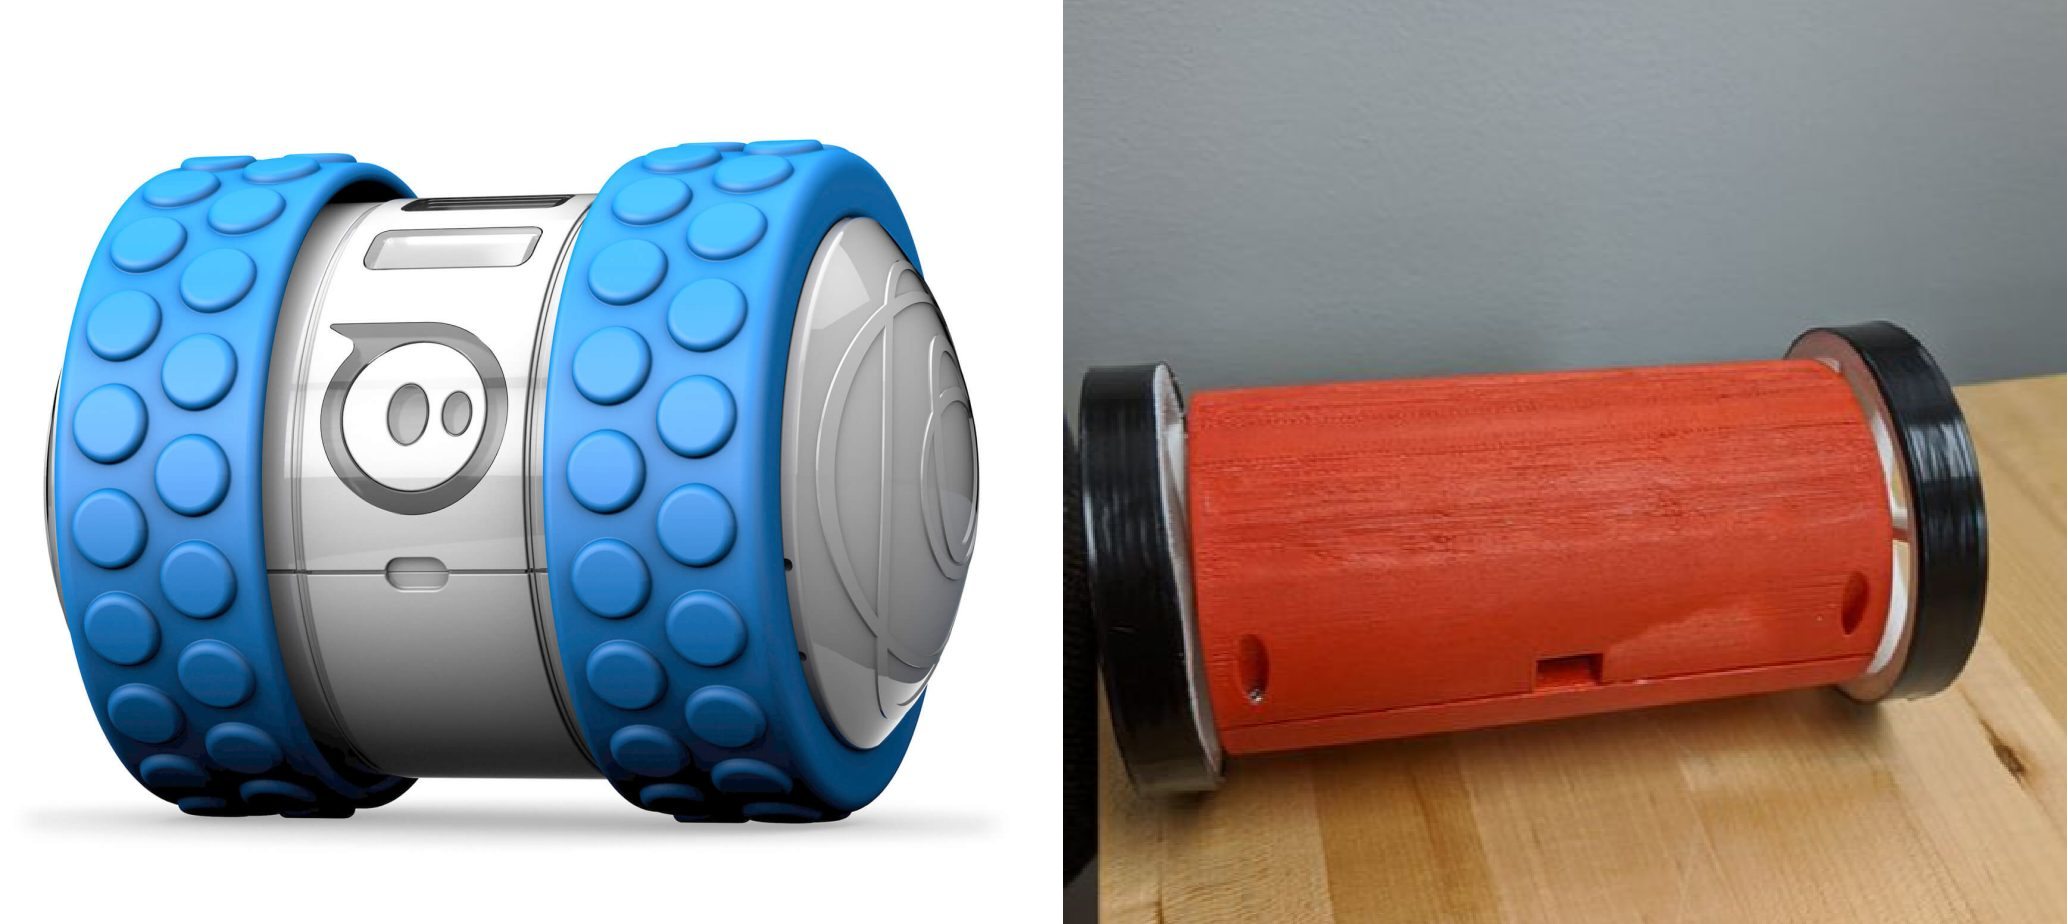
\includegraphics[width=0.5\textwidth]{images/SideBySide.png}
\caption{The Ollie from Sphero comparied with our Design\\Source: Adapted from \cite{ollie:19}}
\label{Ollie}
\end{figure}


\section{Project Implementation}
%Project Implementation (The details of what you did, what you used, and why you made the choices you did. This is likely to be by far the largest section of your report, and can have multiple sub-sections) 

The central piece of the game is the Game Hub. This Hub is constructed with a Raspberry Pi 3 B+ which included enough features to make the gameplay possible. The robots are PCBs and DC Motors wrapped in a 3D printed shell. Each PCB receives commands from the Game Hub via WiFi. Players control each robot with the use of a Wii Balance Board which is connected to the Hub through Bluetooth. The web camera is connected to the Game Hub with USB and detects the unique color of each robot. The play area is a 4ft round surface in which the robots are able to move around and play. The camera sits above the play area on an 8ft post. Each component of the project is described in more detail below. 

\subsection{The Game Hub}

We utilized a Raspberry Pi 3 B+ as our game hub. The device contained both Bluetooth and WiFi capabilities which was critical for communicating to the external game peripherals. The Pi was an excellent choice as it is small, portable, and capable enough to handle the software required for the game. 

The controllers were connected to the Game Hub via Bluetooth. The controllers are based on Wii Balance Boards. The Game Hub starts the controller logic in a separate thread and once connected, continuously polls the Bluetooth devices to ensure they stay connected. When a game is in progress, the data collected from Bluetooth is processed. Once processed, the Game Hub will determine in which direction the player is leaning and send the corresponding command to the player's robot.

\subsection{Controllers}
For our controllers, we used the Wii Balance Board. Our intention behind this controller system was to add layers of complexity and extra challenges to gameplay. The interface was an opensource library found on github. There were a few versions of the library but we electected to use the library written in Python. We made an API for our purposes to be as simple as possible with only two functions that connected to a board and collected the data from the board.

Our API relied on a single WiiController object that connected to multiple boards. The functions of the API are start and get\_data. The start function accepts the MAC Address of one of our boards and instantiated the board to a corresponding WiiBoard object board1, board2, board3, or board4. Once connected, the board will need to be continously polled to ensure the Bluetooth stayed connected. The get\_data function accepts the MAC Address of one Balance board and an array of that board's data would be returned to the Hub. The Hub then processes this data and sends the proper commands to the corresponding robot.

\subsection{Robots}

The robots are a mix of hardware and software. A PCB lies within each robot that contains an ESP-12F. The ESP-12F runs custom software that drives the robot. We printed custom shells and wheels to protect and drive the robots. The custom hardware and software made debugging the robots a challenge but a worthwhile effort nonetheless. 

\begin{figure}[H]
\centering
\captionsetup{justification=centering}
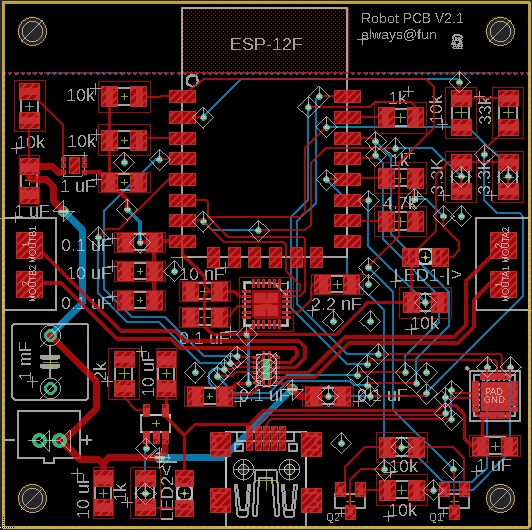
\includegraphics[width=0.5\textwidth]{images/FinalPCB.jpg}
\caption{The custom PCB that controls each robot}
\label{PCB}
\end{figure}

The custom hardware lies in the PCB which can be seen in Figure \ref{PCB}. The PCB contains 4 mounting pads, 2 for each DC Motor that drives the robot, as well as M2.5 drill holes on each corner. The drill holes allowed for the PCBs to be mounted within the shell as seen in Figure \ref{robot}. The ESP-12F chip on the PCB was programmed with the use of USB and a CP2104 programmer chip on the board. An MPU is located in the center of the PCB. The MPU was integrated as a backup to the camera detection. The data from the MPU would allow us to determine if the robot had fallen from the board. This was later discarded as our Computer Vision portion of the project worked as expected. A DRV Motor Driver is included on the PCB to allow for the DC Motors to spin both forward and backward. A LDO chip was also added to handle voltage dropouts. 

The software in the ESP-12F is responsible for receiving data from the Game Hub via WiFi and converting that data to voltages delivered to the DC Motors.  

\begin{figure}[H]
\centering
\captionsetup{justification=centering}
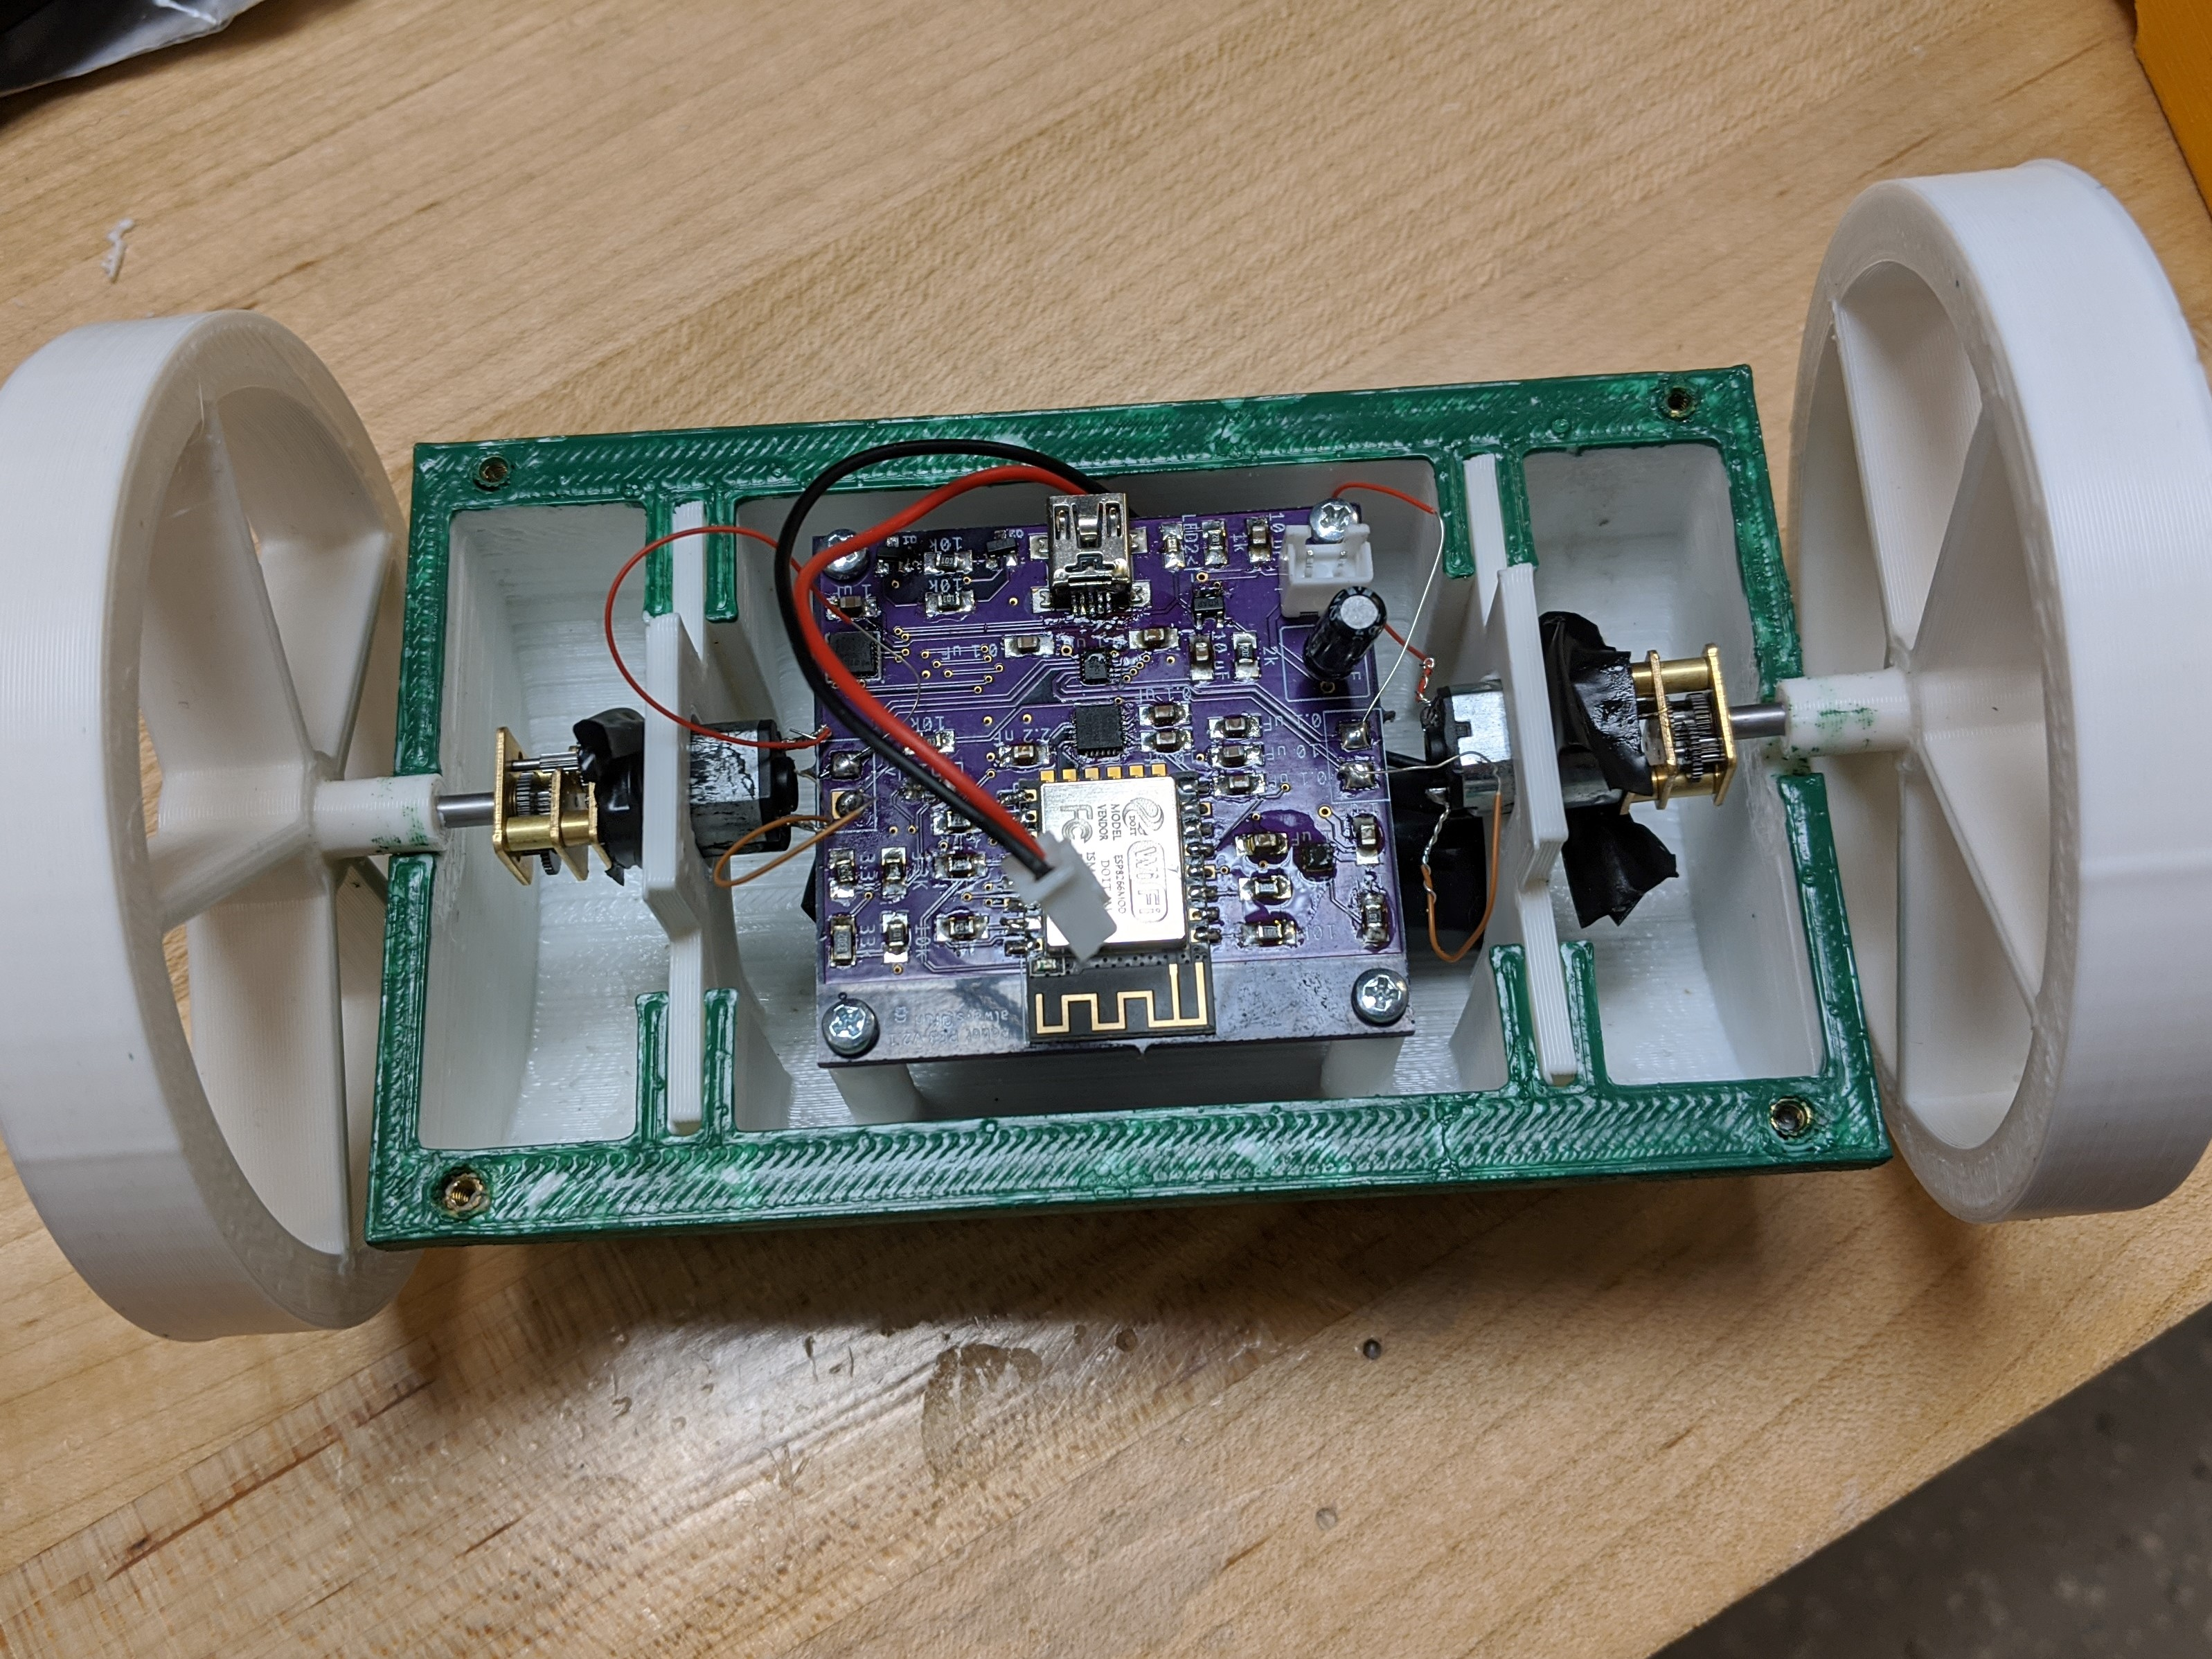
\includegraphics[width=0.5\textwidth]{images/FinalRobot.jpg}
\caption{The finalized robot components in shell}
\label{robot}
\end{figure}

\subsection{The Camera}

The camera used for the project was a Logitech web camera. We considered the Pi Camera as well for the camera but proved to be unreliable. Our first experiment with the Pi Camera ended up shorting something out in the circuitry and our first Raspberry Pi was inoperable. The Pi Camera did offer faster operating speed as the USB interface was bypassed but we elected to use the Logitech camera. We used a 12ft male-to-female USB extension cable which allowed for the camera to rest on top of the camera perch and not the entire Raspberry Pi system which allowed us to easily use the Pi on a nearby table. After a few tests conducted with the camera and OpenCV, any fears of latency were soon removed as the camera proved to be an easy to use asset perfect for the job.  

\subsection{The Play Area}

The play area is simple in nature but plays an essential part in the overall game. We painted the table top white. The floor we were working on caputured the carpet as black, avoiding a need to place a black sheet as the backdrop. As described in the camera section, every color that would enter the black region would be filtered out, meaning once the robot was off the white play area, it turned off and was unable to accept user input. The most complex piece of the play area was the 8ft pole which held the camera. Figure \ref{area} shows how high up the camera needed to rest in order for the entire play area to be seen. It was essential the camera be at this height as to ensure all robots in the area would be captured. We were lucky enough to get a table that sat off the ground enough so that once a player was out, they could not reenter if a glitch with the Computer Vision were to occur. Though this proved to be a nonissue, it was reassuring to have a backup in the worst case scenario. 

\begin{figure}[H]
\centering
\captionsetup{justification=centering}
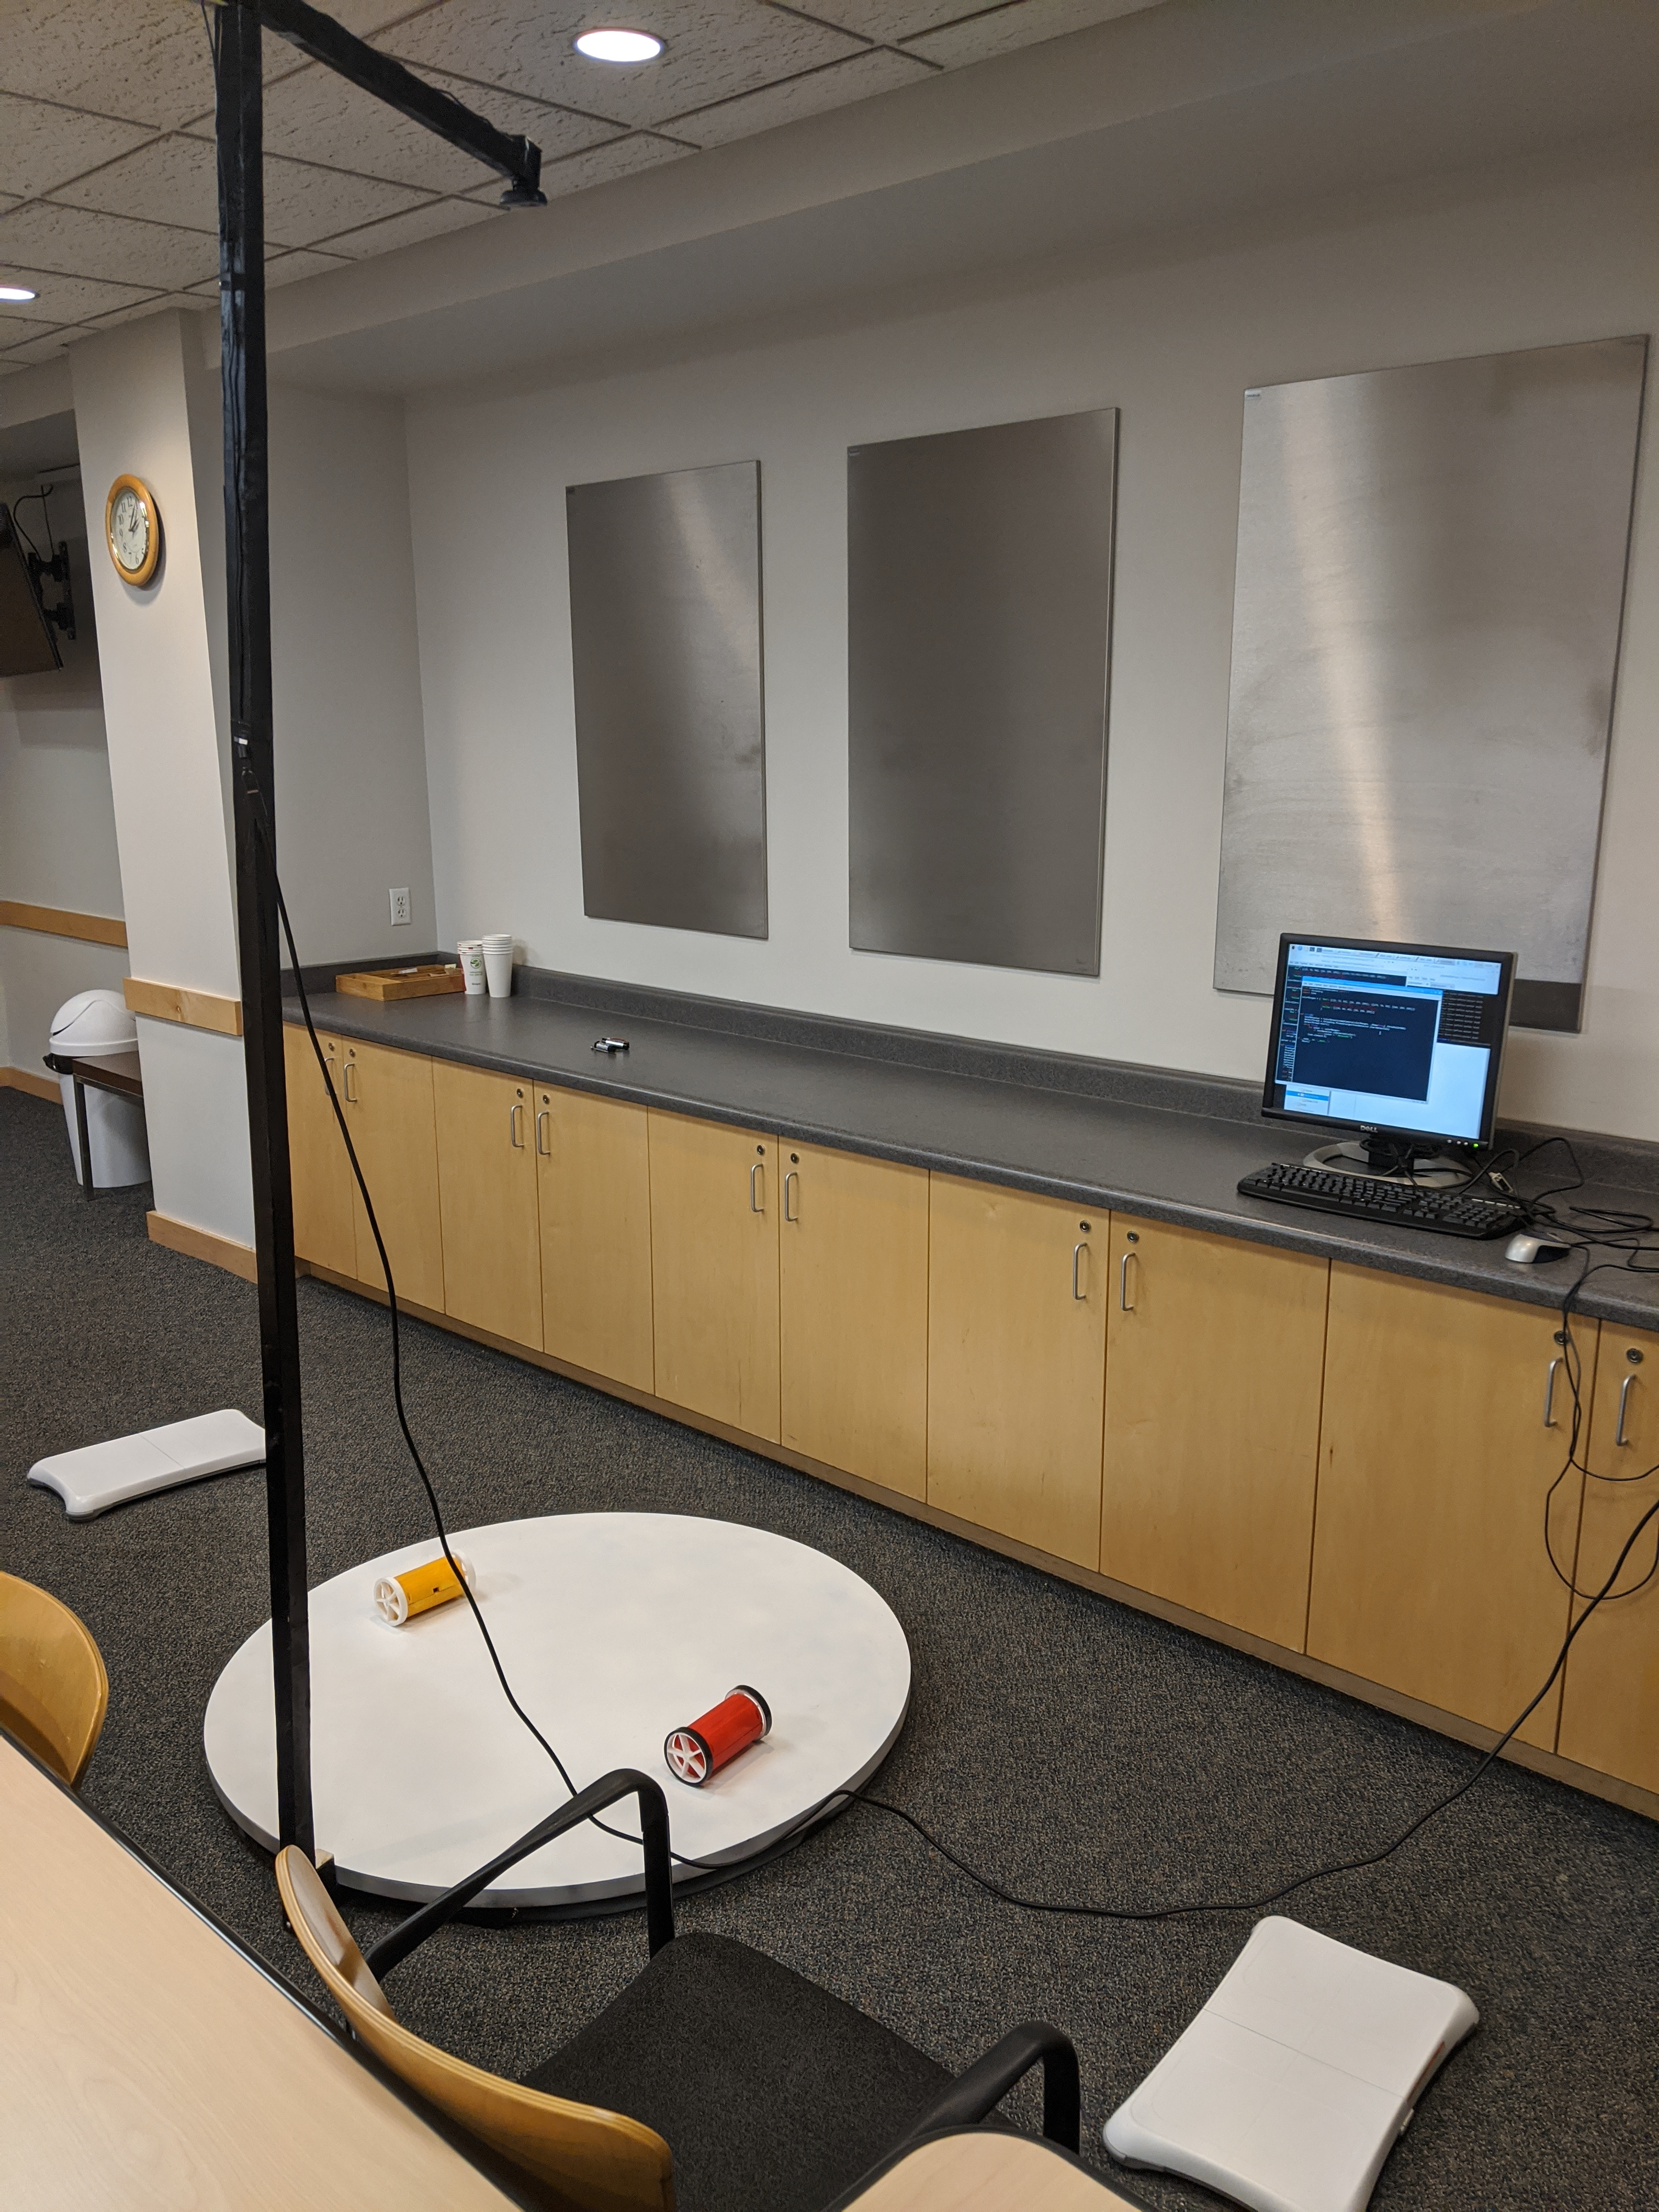
\includegraphics[width=0.5\textwidth]{images/PlayArea.jpg}
\caption{The constructed play area}
\label{area}
\end{figure}

\section{Discoveries}
%Discoveries and pitfalls (things you learned and things that other groups would find helpful)

We learned pretty quick that the original DC motors we were using were far too powerful for such a small play area. The motors offered over 1000 RPM which can be handled with gearing the motors. The unfortunate result of this, however, was the small area in which the gears were to fit. The first few attempts at gearing the motors were a success in many ways and a failure in others. The gears did work and we were able to get a simple gear test box working as seen in Figure \ref{gears}. The gears faced problems with proper meshing, resulting in small pieces of PLA to fly from the test box. With lubrication, the problem continued still. We also attempted acrylic gears as a laser cutter was able to make more precise cuts, allowing the gears to mesh better. Similar problems persisted with acrylic gears as well and any lubrication on the acrylic gears proved to be fruitless. 

\begin{figure}[H]
\centering
\captionsetup{justification=centering}
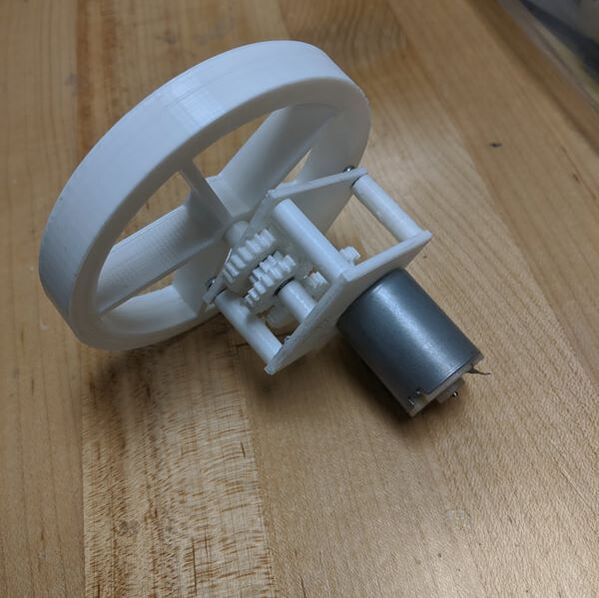
\includegraphics[width=0.5\textwidth]{images/GearTest.jpg}
\caption{The first ideration of the designed gears}
\label{gears}
\end{figure}

The biggest shortcoming we encountered was not developing a prototype in early November. We ordered some of the pregeared motors in October and elected to go with the more powerful motors that required custom gearing to work. In retrospect, we saw that even though we did not intend to go with the pregeared motors, we could have and should have created a prototype with the pregeared motors to test the game area, controllers, and OpenCV with a working robot. This would have also saved time after determining that the custom motors would not work as  expected. 

\section{Evaluation}
%How well did it work - be honest here - if there were things that didn't work out the way you expected, write about them too. Also make sure to describe your testing and evaluation strategy. Don't just say it worked - describe how you know it worked, and even what "worked" means. This is likely to be the second-largest section in your report.

Despite any setbacks and initial concerns, the project was a huge success. While we were not able to accomplish all of our stretch goals, the most basic of play modes was achieved and everyone at the Demo Day had fun playing the game. There were many areas of the project that had unique hang-ups, challenges, and roadblocks. Some of these we were able to solve with little to no issue, others took some time, and the leftovers were abandoned. The next section will cover aspects of the project that worked well and others that are now dead in the water.

The gears are among the greatest achievements and failures of the project. If they had succeeded, the robots would have had more power, leading to harder collisions and potentially more intense games. After a few tests with a completed robot with the custom gears, we soon discovered that the gears proved to be unreliable. The lubrication did stop the gears from heating up and melting but the inconsistent gear meshing led to an unsuccessful implementation. While testing the custom geared robots, the gears would not always turn and got stuck easily. This would have been a disaster during Demo Day. After a few days of trying to solve the issue and attempting to make acrylic gears, we decided to ditch the gears and use pregeared DC Motors. The pregeared motors did not offer the same power but they were able to get the robots moving consistently. The gears were devastating to the project and is the main reason why our stretch goals were not met.

The gears not only cost us extra time, it cost us extra money. The original motors purchased totaled at \$X.XX. With it, brass rods were required along with lubricant. Once acrylic gears were tried, three acrylic sheets were puchased, totalling around \$16. The gears required several iterations of shell components which created a major loss of our PLA filament. With the excess filament, we could have increased the amount of players on the board. The original motor and gear scheme took up a lot more room than the later design, leading to larger shells which required more filament. The gears did end up costing us more but fortunately the expenses were not too excessive.

Despite the gears being a loss, the design of the shell proved to be a success. The design was modular in nature. As can be seen in Figure \ref{shell}, there are inserts for the gear plates that were later modified to suit the needs of the pregeared motors that were used in the final design. The batteries used in the shells weighted it down enough to prevent the body of the shell from excess rotation. Though the body still rotates, it has proved to be a fun "feature, not a bug" game mechanic. Ramps were also added to fit in where the square hole was that was originally designed for USB cable insertion. This was a fortunate coincidence for us as the ramps prevented the robots from rotating the body forward and also added an extra game mechanic, allowing to move robots from the side and not the only the front. The wheels required a small piece of electric or duct tape for good traction on the play area. Fortunately, the cost of the shell was limited to the cost of the PLA filament which totaled no more than \$40. The shell was designed well and the modular design saved us as many changes were made later in timeline. 

\begin{figure}[H]
\centering
\captionsetup{justification=centering}
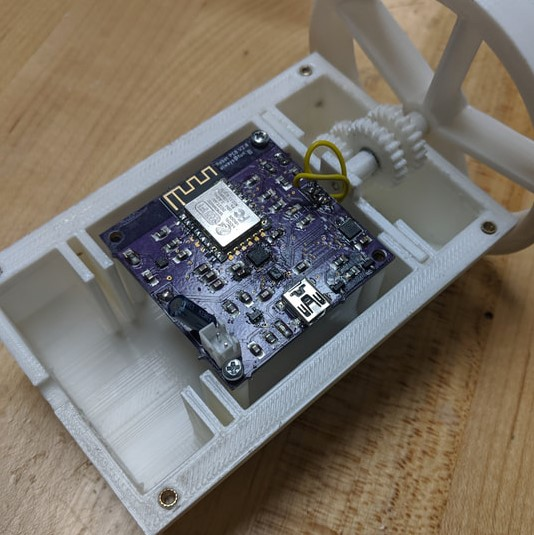
\includegraphics[width=0.5\textwidth]{images/Shell.png}
\caption{A snapshot of the insides of the original robot shell with gears}
\label{shell}
\end{figure}

The PCBs used for the project were well designed with each iteration and worked well every step of the way. The first PCB was designed in April, right before our planning phase was complete. This preliminary PCB was equipped with pinheaders (absent in later models) to debug the design. This worked in our favor as we discovered that the MPU held some pins low by default which prevented the ESP-12F from powering up. We were able to make this discovery by utilizing I2C to communicate with the chip and turn the pin to high to activate the ESP-12F. The second PCB corrected this by removing the connection of that pin to the ESP-12F. This was a trade off as we were no longer able to receive interrupts from the MPU. The second PCB also contained drill holes for mounting the PCBs into the robot shells. The third and final PCBs were very similar to the second with a few parts moved around to ensure each component was clear of the screws in the drill holes. The PCB, while a tedious task to solder, was one of the most successful components of the project.  

The Raspberry Pi was a very useful aspect to the project, allowing us to use free and open source libraries, but we were ill prepared for the issues it came with. The Raspberry Pi worked very well for our needs and the multicore processing power helped the game logic run smoothly. Melvin was able to enable threading so the Bluetooth controllers, WiFi, game logic, and camera/OpenCV interface ran seamlessly. We were unaware of the poor power protection provided by the Raspberry Pi hardware. The first Raspberry Pi was fried after the Pi Camera drew too much current which also broke the Pi Camera. We assumed incorrectly that the Raspberry Pi would have a robust power protection scheme. The second Raspberry Pi was fried for unknown reasons. The third Raspberry Pi fried when two GPIO pins shorted to one another. Once we discovered how vulnerable the Raspberry Pi's are, we treated the last with extra special care. The final Raspberry Pi was to remain in the casing and only be connected to anything via USB, HDMI, and the official Raspberry Pi power supply. Once these issues were all sorted out, we treated it as delicately as a newborn baby. We were on the verge of porting all of the code to someone's laptop but the laptop would require running Linux as all of our Raspberry Pi code works only on Linux libraries. This would have been an even larger upset so we decided to keep with the Raspberry Pi and we fortunately found out all potential power issues and it suited our needs. 

The Wii Balance Boards made the game play a lot more fun than intended. When selecting our controllers in our initial proposal, we stated concerns about multiple Bluetooth objects in a single area creating a lot of noise. This proved to be a nonissue as there were little to no issues with interfacing with the Wii Balance Boards. We used a simple control scheme to make the game play intuitive, fun, and exciting. When a player leans forward, the robot moves forward. When the player leans back, the robot moves back. When leaning left and right, the robot would only rotate in that direction. This added some extra strategy from a player standpoint. Players need to now think a few moves ahead to ensure that they will not be vulnerable when needing to move right or left. The controllers proved to be a vital component that made the game so enjoyable.

The use of WiFi and Bluetooth to control the game was a huge success. During our presentation, we noted that were was a lot of potential for noise interference and latency issues. Fortunately we did not encounter any of these issues. The response time from controller input to robot movement was so good there was hardly any latency observed. The response time of the camera and OpenCV was also fast enough that when a robot left the arena, it was immediately turned off. 

\section{Bill of Materials}
% Bill of materials (or at least a list of all the materials, equipment, etc. that you used. You don't need prices here, but you should include a list of things you used)

Our project cost a whopping 900 dollary doos!

\section{Conclusion}
%- Conclusions (wrap things up with some final text. Include a pointer to your final web site.) 

Our senior project proved to be a huge success and we learned many valuable lessons from it. We were able to work the first three months of the semester in parallel which resulted in rapid development. We began integrating around November and had it finalized just in time to present at Demo Day. The project milestones and meeting logs can be found at http://bumpercarsumo.weebly.com/.

\bibliographystyle{IEEEtran}
\bibliography{IEEEabrv,bib/ref}

\end{document}